% These are the lecture notes for my CSCI360 course SPRING 2017
% at John Jay College of Criminal Justice.

% Feel free to edit these slides and use them for your own courses.
% HOWEVER DO NOT REMOVE THESE LINES!
% Email me at: awood [at] jjay.cuny.edu
% or at: awood [at] gradcenter.cuny.edu


\documentclass{beamer}

\usepackage{tikz}
\usetikzlibrary{calc}

\usepackage{forest}
\usepackage{verbatim}
\usepackage{color}


\setbeamertemplate{footline}[frame number]
\setbeamertemplate{navigation symbols}{} 

\newtheorem{thm}{Theorem}[section]
\newtheorem{lem}{Lemma}
\newtheorem{cl}{Claim}
\newtheorem{cor}{Corollary}[section]
\newtheorem{conj}{Conjecture}
\newtheorem{quest}{Question}
\newtheorem{defn}{Definition}[section]
\newtheorem{obs}{Observation}[section]
\newtheorem{exam}{Example}

\newcommand{\im}{\operatorname{im}}
\newcommand{\id}{\operatorname{id}}
\newcommand{\interior}{\operatorname{int}}
\newcommand{\bdry}{\operatorname{bdry}}
\newcommand{\<}{\langle}
\renewcommand{\>}{\rangle}
\newcommand{\Gab}{(G_\phi)^{ab}} 
\newcommand{\phibar}{\bar{\phi}}
\newcommand{\Z}{\mathbb{Z}}
\newcommand{\N}{\mathbb{N}}
\newcommand{\Q}{\mathbb{Q}}
\newcommand{\R}{\mathbb{R}}
\newcommand{\C}{\mathbb{C}}
\newcommand{\A}{\mathcal{A}}
\newcommand{\OO}{\mathcal{O}}
\newcommand{\UU}{\mathcal{U}}
\newcommand{\power}{2^{\{P_1, \cdots , P_n\}}}
\newcommand{\bp}{\begin{problem}}
\newcommand{\ep}{\end{problem}}
\newcommand{\ba}{\begin{answer}}
\newcommand{\ea}{\end{answer}}
\newcommand{\ds}{\displaystyle}
\newcommand{\ben}{\renewcommand{\theenumi}{\alph{enumi}}
\renewcommand{\labelenumi}{(\theenumi)}\begin{enumerate}}
\newcommand{\een}{\end{enumerate}}
\newcommand{\Hess}{\operatorname{Hessian}}
\newcommand{\Aut}{\mathrm{Aut}}
\newcommand{\Inn}{\mathrm{Inn}}
\newcommand{\Out}{\mathrm{Out}}
\newcommand{\End}{\mathrm{End}}


\mode<presentation>
{
%  \usetheme{default}
  \setbeamercovered{invisible}
}


\usepackage[english]{babel}
\usepackage[latin1]{inputenc}
\usepackage{times}
\usepackage[T1]{fontenc}
\usepackage{stmaryrd}

%\usetheme{default}
%\usetheme{AnnArbor}
%\usetheme{Antibes}
%\usetheme{Bergen}
%\usetheme{Berkeley}
%\usetheme{Berlin}
%\usetheme{Boadilla}
%\usetheme{CambridgeUS}
%\usetheme{Copenhagen}
%\usetheme{Darmstadt}
%\usetheme{Dresden}
%\usetheme{Frankfurt}
%\usetheme{Goettingen}
%\usetheme{Hannover}
%\usetheme{Ilmenau}
%\usetheme{JuanLesPins}
%\usetheme{Luebeck}
%\usetheme{Madrid}
%\usetheme{Malmoe}
%\usetheme{Marburg}
%\usetheme{Montpellier}
%\usetheme{PaloAlto}
%\usetheme{Pittsburgh}
%\usetheme{Rochester}
\usetheme{Singapore}
%\usetheme{Szeged}
%\usetheme{Warsaw}

%\usecolortheme{default}
%\usecolortheme{albatross}
\usecolortheme{beaver}
%\usecolortheme{beetle}
%\usecolortheme{crane}
%\usecolortheme{dolphin}
%\usecolortheme{dove} % grey, white, yellow
%\usecolortheme{fly} %grey, yellow
%\usecolortheme{lily} %white, yellow, blue
%\usecolortheme{orchid}
%\usecolortheme{rose}
%\usecolortheme{seagull}
%\usecolortheme{seahorse}
%\usecolortheme{whale}
%\usecolortheme{wolverine}

% Title page

\title[CSCI360]{Ciphers}

\subtitle{Caesar's Shift}

\author
{Lecture notes of Alexander Wood \\ CSCI 360 Cryptography and Cryptanalysis \\ \scriptsize \href{mailto:awood@jjay.cuny.edu}{awood@jjay.cuny.edu}}
\institute[JJay]{John Jay College of Criminal Justice}  

\date{}

\begin{document}

% Remove 'figure' text from figure captions 
\setbeamertemplate{caption}{\raggedright\insertcaption\par}

\begin{frame}
  \titlepage
\end{frame}


\begin{frame}
\frametitle{Caesar's Shift}

The first cryptosystem we will look at is called \textbf{Caesar's Shift}. This cipher is one of the earliest ever invented -- it was used by Julius Caesar to disguise communication!
\end{frame}


\begin{frame}
\frametitle{The Original Cipher}

In Caesar's original cipher, every letter was shifted exactly three letters to the right. Note that X, Y, and Z are brought around to the beginning and shifted to A, B, and C, respectively.
\begin{figure}
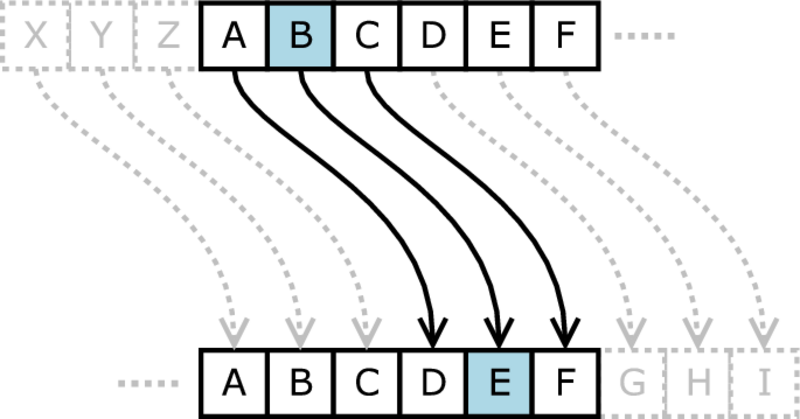
\includegraphics[scale=.3]{IMG/fig1.png}
\end{figure}
\end{frame}

\begin{frame}
\frametitle{The Original Cipher}

This is perhaps better visualized as a circle! In this photo, the plaintext is on the outside, and the ciphertext is on the inside. To encrypt a phrase, match each letter on the outside to a letter on the inside. To decrypt, match each letter on the inside to the corresponding letter on the outside. 
\begin{figure}
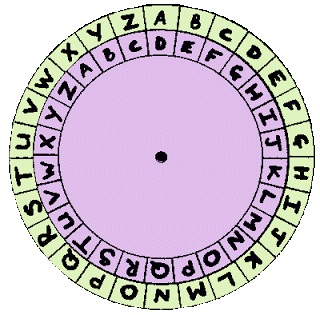
\includegraphics[scale=.3]{IMG/wheel.jpg}
\caption{\tiny Image from \url{http://dubworks.blogspot.com/2013/10/some-exercises-with-caesar-cipher-with_22.html}}
\end{figure}
\end{frame}


\begin{frame}
\frametitle{Exercise 1}

Use the wheel below to decrypt the message: 
\begin{center}
KRWOLQH EOLQJ
\end{center}
\begin{figure}
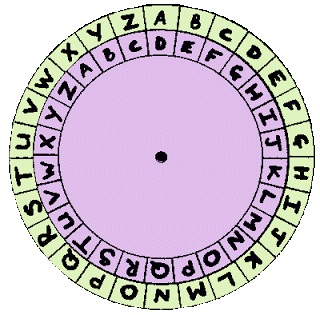
\includegraphics[scale=.5]{IMG/wheel.jpg}
\end{figure}
\end{frame}

\begin{frame}
\frametitle{Shift Ciphers}

Of course, we can also shift the alphabet differently! Instead of shifting three letters, we could shift seven, or twenty, or fifteen!
\end{frame}


\begin{frame}
\frametitle{I Got The Keys}

Let's call Caesar's original cipher a \textbf{3-shift}, because we shifted each letter three to the right. 

\begin{figure}
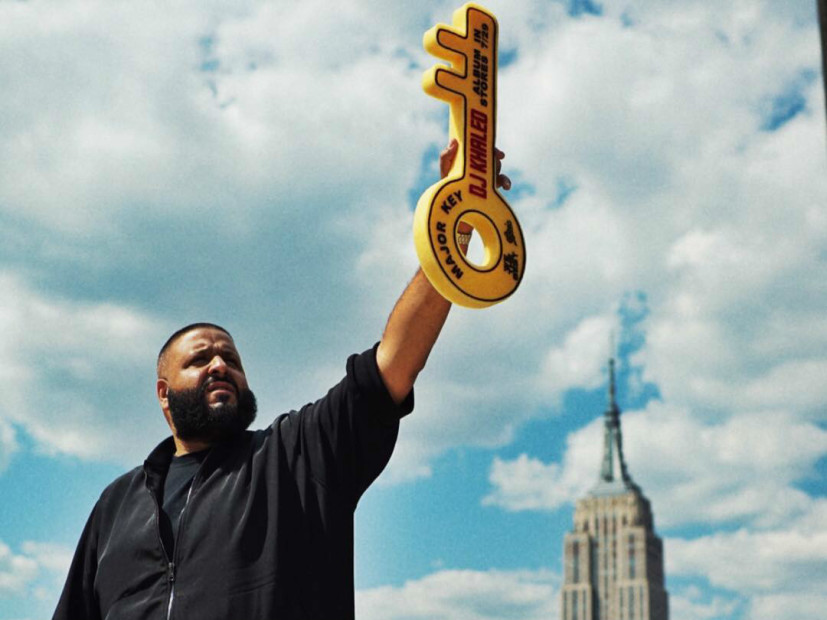
\includegraphics[scale=.18]{IMG/keys.jpg}
\caption{\tiny keys, keys, keys}
\end{figure}
How many different possible shifts are there?
\end{frame}

\begin{frame}
\frametitle{Keys and Keyspaces}

The \textbf{keyspace} of the shift cipher is 25, and the key is a number in the range 1 through 25. 
\end{frame}

\begin{frame}
\frametitle{Exercise 2}

Say the key is $K = 19$, with a shift corresponding to the wheel below. 
\begin{figure}
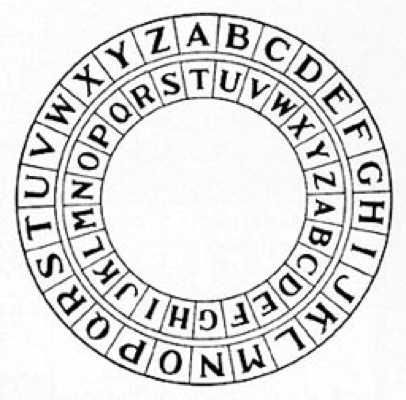
\includegraphics[scale=.3]{IMG/wheel2.jpg}
\end{figure}

What is the decryption of IHDXFHG?
\end{frame}


\begin{frame}
\frametitle{Exercise 3}

Use a Caesar's Cipher Encypter at 
\begin{center}
\url{https://lingojam.com/CaesarCipher}
\end{center}

Go ahead and encrypt any message you want! 
\end{frame}

\begin{frame}
\frametitle{Exercise 4}

Use the Caesar's Cipher Decrypter at
\begin{center}
\url{http://www.mygeocachingprofile.com/codebreaker.caesarcipher.aspx}
\end{center}

To decrypt the following phrases and keys:
\begin{enumerate}[(a)]
\item
TSOIFEPP KS, $K=4$

\item 
PK XA KN JKP PK XA PDWP EO PDA MQAOPEKJ, $K=22$

\item 
JYV JVCCJ JVRJYVCCJ SP KYV JVRJYFIV, key unknown!
\end{enumerate}
\end{frame}

\begin{frame}[fragile]
\frametitle{Coding Exercise 1: Caesar's 3-Cipher}

First, let's use Python to encrypt using Caesar's original cipher, which shifts every input three letters to the right. Let's write a function called \verb|encrypt| which encrypts using Caeser's 3-cipher, as well as a corresponding \verb|decrypt| function.
\end{frame}

\begin{frame}[fragile]
\frametitle{Coding Exercise 1: Caesar's 3-Cipher}

Write Python code for the following functions using Caesar's 3-shift.  
\begin{verbatim}
encrypt
INPUT: plaintext string
OUTPUT: ciphertext string

decrypt
INPUT: ciphertext string
OUTPUT: plaintext string
\end{verbatim}
\end{frame}


\begin{frame}[fragile]
\frametitle{Coding Exercise 2: Shift Cipher}

Now let's code the shift cipher with \emph{any} key. Our functions \verb|encrypt| and \verb|decrypt| must now take on a second argument, \verb|key|.
\end{frame}


\begin{frame}[fragile]
\frametitle{Coding Exercise 2: Shift Cipher}

Write Python code for the following functions using the shift cipher.
\begin{verbatim}
encrypt
INPUT: plaintext, key
OUTPUT: ciphertext

decrypt
INPUT: ciphertext, key
OUTPUT: plaintext
\end{verbatim}
\end{frame}


\begin{frame}
\frametitle{References}

\begin{itemize}
\item Caesar's Shift Encrypter: \url{https://lingojam.com/CaesarCipher}
\item Caesar's Shift Decrypter: \url{http://www.mygeocachingprofile.com/codebreaker.caesarcipher.aspx}
\item The Assigned Reading: Schneier's \emph{Applied Cryptography} pages 10-13
\item Our other textbook \emph{Invent With Python} has a chapter on Caesar's cipher with another Python implementation: \url{http://inventwithpython.com/hacking/chapter6.html}
\item C++ and Java implementations: \url{http://www.geeksforgeeks.org/caesar-cipher/}
\end{itemize}
\end{frame}
\end{document}


